%  FICHIER  :   template_fira_two_cols.tex
%  A copier à côté des autres .tex et à déclarer dans config.json
% ------------------------------------------------------------------
\documentclass[11pt,a4paper]{article}

% ─── pack de base ─────────────────────────────────────────────────
\usepackage[T1]{fontenc}
\usepackage[utf8]{inputenc}
\usepackage{textcomp}
\usepackage{newtxtext}
\usepackage[british]{babel}
\usepackage[left=0mm,right=0mm,top=0mm,bottom=0mm]{geometry}
\usepackage[stretch=25,shrink=25,tracking=true,letterspace=30]{microtype}
\usepackage{graphicx,xcolor,marvosym,enumitem,paracol,hyperref}
\usepackage{FiraSans}
\renewcommand{\familydefault}{\sfdefault}
\usepackage{array} 
\usepackage{tabularx}
\usepackage{ragged2e}
 \usepackage{fontawesome}
% ─── couleurs & listes ────────────────────────────────────────────
\definecolor{cvblue}{HTML}{304263}
\setlist{parsep=0pt,topsep=0pt,partopsep=1pt,itemsep=1pt,leftmargin=6mm}
\hypersetup{colorlinks=true,urlcolor=white,linkcolor=white}

% ─── macros maison (identiques au modèle original) ────────────────
\newcommand{\dates}[1]{\hfill\textbf{#1}}
\newcommand{\is}{\par\vskip.5ex plus .4ex}
\newcommand{\smaller}[1]{{\small$\diamond$\ #1}}
\newcommand{\headleft}[1]{\vspace*{3ex}\textsc{\textbf{#1}}\par%
  \vspace*{-1.5ex}\hrulefill\par\vspace*{0.7ex}}
\newcommand{\headright}[1]{\vspace*{2.5ex}\textsc{\Large\color{cvblue}#1}\par%
  \vspace*{-2ex}{\color{cvblue}\hrulefill}\par}

% ─── défaut de secours si sidetext absent dans d’autres modèles ───
\providecolor{sidetext}{rgb}{0,0,0}
\definecolor{maincolor}{HTML}{ffffff}
% ─────────────────────────── DOCUMENT ─────────────────────────────
\begin{document}
\thispagestyle{empty}
\setlength{\topskip}{0pt}\setlength{\parindent}{0pt}\setlength{\parskip}{0pt}
\raggedbottom

\begin{minipage}[t]{0.33\textwidth}
  % Bande bleue d’en-tête
  \colorbox{cvblue}{\begin{minipage}[t][5mm][t]{\textwidth}\null\end{minipage}}
  \vspace{-.2ex}
  \colorbox{cvblue!90}{%
    \color{white}\kern0.09\textwidth
    \begin{minipage}[t][293mm][t]{0.82\textwidth}\raggedright
      \vspace*{2.5ex}
      % -------- Identité ------------------------------------------
      \Large Judikael Mourouvin\normalsize

      % Photo (s’affiche seulement si d75cfa1b43a548778ea3bc489af73f0f.png ≠ vide)
      \ifx\relaxd75cfa1b43a548778ea3bc489af73f0f.png\relax\else
        \vspace{2ex}\null\hfill
        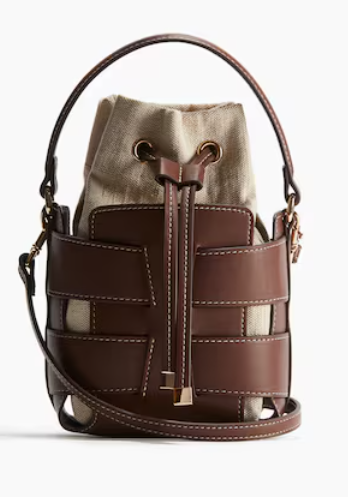
\includegraphics[width=0.65\textwidth]{d75cfa1b43a548778ea3bc489af73f0f.png}
        \hfill\null
      \fi

      % -------- Profil -------------------------------------------
      \headleft{Profil}
      \begingroup           % ouvre un groupe local
       \justifying         % rétablit la justification pleine
        Passionné par l’informatique et le marketing digital, je maîtrise la configuration de postes, la maintenance et le diagnostic d’incidents. Mon année d’alternance à la DSI de la mairie du Gosier m’a permis de piloter des projets numériques et d’accompagner les utilisateurs au quotidien. Polyvalent et rigoureux, je conjugue compétences techniques et sens du service pour optimiser l’environnement informatique. Je souhaite désormais mettre ces atouts au service d’une équipe dynamique à temps plein.
      \endgroup             % referme : on revient à \raggedright

      % -------- Contact ------------------------------------------
      \headleft{Contact}\small
      \MVAt\  \texttt{jkmou971@gmail.com}\par
      \Mobilefone\ +590 0690 91 14 48\par
      \Letter\ Route de Cocoyer\par
      97190 Gosier\par
      \faLinkedin\  \href{}{}
      \normalsize

      % -------- Langues (si dispo) -------------------------------
      \ifx\relax\begin{itemize}[leftmargin=*]
\item English - \textcolor{gray}{}
\item Espagnol - \textcolor{gray}{}\end{itemize}\relax\else
        \headleft{Langues}
        \begin{itemize}[leftmargin=*]
\item English - \textcolor{gray}{}
\item Espagnol - \textcolor{gray}{}\end{itemize}
      \fi

      % -------- Compétences --------------------------------------
      \headleft{Compétences}
      \begin{itemize}[leftmargin=*]
\item Administration
\item Réseaux
\item Assistance
\item Maintenance
\item Diagnostic
\item Configuration
\item Marketing\end{itemize}

      % -------- Centres d’intérêt --------------------------------
      \headleft{Intérêts}
      \begin{itemize}[leftmargin=*]
\item Lecture
\item Sport
\item Musique
\item Voyage
\end{itemize}

    \end{minipage}\kern0.09\textwidth
  }
\end{minipage}
% ================================================================
\hskip2.5em
% ======================= COLONNE DROITE =========================
\begin{minipage}[t]{0.56\textwidth}
  \setlength{\parskip}{0.8ex}
  \vspace{2ex}

  % ---------- EXPERIENCE ----------------------------------------
  \headright{Expérience}
  \colorbox{maincolor}{%
  \begin{minipage}{\linewidth}
    \noindent
    \textbf{Alternant en marketing digital}\hfill 09/2023 - 08/2024\\
    Mairie du Gosier – DSI\\[-0.3em]
    \begin{itemize}[leftmargin=*]
      \item Coordonné des projets numériques, améliorant les services municipaux. \item Analysé les besoins utilisateurs et déployé des solutions adaptées, réduisant les tickets. \item Assuré le support et animé des formations, renforçant l’autonomie digitale des agents.
    \end{itemize}
  \end{minipage}}

\vspace{3mm}

\colorbox{maincolor}{%
  \begin{minipage}{\linewidth}
    \noindent
    \textbf{Animateur de la zone informatique}\hfill 09/2022 - 08/2023\\
    Pôle emploi, Gosier\\[-0.3em]
    \begin{itemize}[leftmargin=*]
      \item Fourni une assistance technique aux demandeurs d’emploi dans l’espace numérique. \item Configuré et entretenu les postes pour garantir leur disponibilité. \item Diagnostiqué et résolu les incidents, réduisant les temps d’arrêt.
    \end{itemize}
  \end{minipage}}

\vspace{3mm}

\colorbox{maincolor}{%
  \begin{minipage}{\linewidth}
    \noindent
    \textbf{Stagiaire informaticien}\hfill 10/2020 - 06/2021\\
    Numerika, Baie-Mahault\\[-0.3em]
    \begin{itemize}[leftmargin=*]
      \item Installé et configuré les équipements informatiques sur site. \item Assuré le support utilisateurs en résolvant les incidents quotidiens. \item Réalisé la maintenance préventive, prolongeant la durée de vie du parc.
    \end{itemize}
  \end{minipage}}        % ← déjà formaté par build_placeholders()

  % ---------- EDUCATION -----------------------------------------
  \headright{Formation}
  \colorbox{maincolor}{%
  \begin{minipage}{\linewidth}
    \noindent
    \textbf{Bachelor Marketing Digital}\hfill 09/2023 - 08/2024\\
    CFA IUTS\\[-0.3em]
    \begin{itemize}[leftmargin=*]
      \item Marketing numérique, gestion de projet, SEO/SEA, analyse de données.
    \end{itemize}
  \end{minipage}}

\vspace{3mm}

\colorbox{maincolor}{%
  \begin{minipage}{\linewidth}
    \noindent
    \textbf{BTS Systèmes numériques option Informatique et Réseaux}\hfill 09/2019 - 06/2021\\
    Lycée Chevalier Saint-Georges, Abymes\\[-0.3em]
    \begin{itemize}[leftmargin=*]
      \item Architecture systèmes et réseaux, maintenance matériel/logiciel, sécurité et support utilisateurs.
    \end{itemize}
  \end{minipage}}

\end{minipage}

\end{document}
